% !TeX root = ../incremental_SS_Translation.tex
\chapter{Kalpasthāna 8: Poisonous insects}

\section{Introduction} 

This is the last chapter of the \emph{Kalpasthāna}.  Since the
chapter-colophons of the Nepalese manuscripts of the whole
\emph{Suśrutasaṃhitā} commonly end with the statement, “here ends the
\SS\ together with the \emph{Uttaratantra},” we can presume that an older
version of the \SS, sans \emph{Uttaratantra}, ended with the present chapter.
Added to this, the beginning of the next section of the work, the
\emph{Uttaratantra}, reads,
\begin{quote}
It being declared in the preceding 120
chapters, from here on, in the latter section, I shall explain the
meanings in detail, fully.\footnote{Note that this is not the reading
    of the vulgate, which says that the \emph{Uttaratantra} will explain
    everything that was \emph{not} completely explained before.}  Now, I
    shall explain the treatise called “the latter” where diseases
    in their diversity are fully revealed.
    \end{quote}
It is often the case with evolving works that new chapters are added
at the start or, especially, at the end of a work.  This has been true
since the \emph{Ṛgveda}.  The \emph{Kalpasthāna} has a different character
from the rest of the \SS, for example eschewing theoretical
considerations in many situations.  It may therefore itself have once
been an addition to an even earlier medical work consisting of four main
divisions.

\subsection{Insect names}

It is more than usually difficult to equate the Sanskrit names of
insects with contemporary creatures.  In fact, it is mostly
impossible. This is partly, at least, because historical entomology is
non-existent as a discipline. Furthermore, entomology as a science in
South Asia is dramatically undeveloped when compared, for example,
with botany.\footnote{\citet{desm-1992} devoted a book of 368 pages to
    the early history of Indian botany; \citet[338--345]{dove-1922}
    described the history of Indian entomology in seven pages.}  There are
few general surveys of insects in India and virtually none that record
historical names or literary references.  In the twelfth century,
Ḍalhaṇa made the following remark about the commentators who lived
before his time:
\begin{quote}
These different types of insects are not described by commentators
like Suvīra, Nandin,Varāha, Jejjjaṭa and Gayadāsa, so they have to be
identified by people from different
localities.\footnote{\Dalhana{5.8.4}{586}: \dev{ete kīṭakabhedā
    nānādeśīyalokādavagantavyāḥ, yataḥ
    suvīranandivarāhajejjaṭagayadāsādibhiḥ ṭīkākārairna vyākhyātāḥ}.
    (Varāha is called Vārāha by \Dalhana{2.13.3}{318}.) Cf.\
    \tvolcite{IA}[387--388]{meul-hist} on Suvīra and \emph{mutatis
mutandis} on
    the other commentators}
\end{quote}
Thus, even pre-modern Sanskrit authors were not expert regarding the
identities of the insects discussed in the
\SS.\footnote{\cite{moni-sans} includes 191 insect names, almost none
    of which are identified.}  
    
In general the names listed in passages 5--14 are the  least
recognizable.  Most seem never to appear elsewhere in Sanskrit
literature or even elsewhere in the \SS.  The names mentioned from
passages 25 onwards are mostly recognizable and do appear elsewhere
Sanskrit literature.\footcite[E.g.,][]{mitr-2005} This chapter
therefore gives the appearance of having two distinct parts.  First,
there is a taxonomy arranged according to humoral characteristics,
containing otherwise unknown insect names. Second follows a
concatenated treatise with more recognizable ordinary-language
nomenclature coupled with creature-by-creature nosology and therapy.

%\ignoreargument{agniprabhā, agniraja,
%        agnirajas, agnika, apacit, aparājita, abhīrājī, arimedaka, alpaśayu,
%        avamūtrita, avalgulī, avaskaraka, āgneya, āvartaka, indragopa,
%        utkleśaka, uttiṅga, utpādikā, upādika, urabhrasārikā, ṛṇamatkuṇa,
%        ejatka, eṇīpadī, aindrādṛśa, aindrāliśa, kaṇḍūmakā, kambala,
%        karṇakīṭā, karṇakīṭī, karṇasūci, kaṣkaṣa, kaṣāyavāsika, kāṣāyavāsika,
%        kāṣṭhakīṭa, kiṇa, kiṃtanu, kīṭa, kīṭī, kīṭagardabhaka, kīṭāvapanna,
%        kīṭaka, kuṇa, kunta, kumārikā, kumbhin, kumbhīnasa, kuṣumbha,
%        kuṣumbhaka, kṛmi, kṛmikara, kṛmitā, kṛmirāga, kṛmisarārī, kṛṣṇā,
%        kṛṣṇagodhā, kṛṣṇatuṇḍa, keśakīṭa, keśāda, kaiṭa, kokila, koṭika,
%        koṭira, kośakārī, kośastha, kauṇḍilyaka, klīta, kṣārakīṭa, kṣīrakīṭa,
%        khaga, khajyotis, khadyotā, kharju, kharjū, garādhikā, guhyadīpaka,
%        golikā, ghuṇa, ghuṇapriyā, ghuṇavallabhā, ghuṇākṣara, cicciṭiṅga,
%        citraśīrṣaka, cipiṭa, jatukṛt, janturasa, jalamakṣikā, taṇḍurīṇa,
%        tarda, talpakīṭa, tālaka, tuṅganābha, tuṅgīnāsa, tuṇḍikerin,
%        tailakīṭa, toṭaka, trikaṇṭaka, troṭaka, daṃśa, daṃśanāśinī,
%        dadrunāśinī, darbhakusuma, darśanī, divī, dundubhika, dehikā,
%        dyotiriṅgaṇa, dhundhumāra, nīlamīlika, pañcakṛṣṇa, pañcaśukla,
%        pañcāla, pañcālaka, pataṃga, padmakīṭa, pallavita, pākamatsya,
%        pāṭalakīṭa, picciṭa, picciṭaka, pulaka, puṣpakīṭa, pūtikīṭa, pūtyaṇḍa,
%        prajāpati, prabhākīṭa, pralūna, prāvārakīṭa, pluṣi, balabha, bindula,
%        bhadrapīṭha, makara, maṇḍalapucchaka, madyakīṭa, madhukeśaṭa,
%        mayūrikā, yavāṣa, yāva, yevāṣa, raktarāji, raktarājī, raktavarṇa,
%        rasaja, lākṣā, lākṣātaru, lomakīṭa, vajrakīṭa, vaṭi, vaṭibha, vāhaka,
%        vāhyakī, vināsaka, vināsika, vināsikā, vicilaka, viḍbhuj, vedamukhya,
%        vaidala, śakragopa, śakragopaka, śakunta, śatadāruka, śatapattraka,
%        śambuka, śaluna, śādvalābha, śūkā, śūkadoṣa, śūkavṛnta, śūrakīṭa,
%        śvetakṛṣṇā, ṣaṭpada, ṣaḍbindu, ṣaḍvindhyā, sarabhaka, sarāva,
%        sarvaśvetā, sarṣapakī, sarṣapika, sārikāmukha, simīka, sīmika,
%        sūkṣmatuṇḍa, sūkṣmaṣaṭcaraṇa, sūcīmukha, sūcīka, saukṣmaka, saurasa,
%        sauvarṇikā, halagolaka, hastikakṣa}

\subsection{Literature} A brief survey of this chapter's contents and
a detailed assessment of the existing research on it to 2002 was
provided by Meulenbeld.\footcite[IA, 296--299]{meul-hist} 

The early history of entomology in India was fragmented until the
study of \citet{maxw-1909} who provided a comprehensive and well
illustrated reference compendium. \citet{dove-1922} gave an overview
of the early years of the field, though he admitted that, “I have not
the linguistic attainments to discuss the mention of various insects
in ancient Sanskrit works.”   Entomological studies focussed on south
India include those of \citet{bain-1914} and \citet{rama-1963}.
\tvolcite{IB}[402]{meul-hist} provided short bibliographies on Indian
scorpions (note 214) and on spiders (note 222). Some insects were
included by \citet{ball-1888} in his study of the Indian flora and fauna
known to classical Greek authors. \citet{kaur-2018} provided a unique
but very brief historical sketch of some arthropod references in
Sanskrit literature.

\newpage
\section{Translation}



\begin{translation}

\item[1]
 And now I shall explain the \se{kalpa}{procedure} about 
 insects\sse{kīṭa}{insect}.
 

\subsection{Taxonomy of insects}

%\item[3--17ab] 

\item [3] 

Insects originate from snakes' semen, feces, urine, the rot of corpses,
and eggs.\footnote{\tvolcite{3}[78]{shar-1999} omitted “snakes'\,” making it 
sound as if insects are just born of any semen, etc.}  Their
\sse{prakṛti}{character}characters are traditionally divided
into \diff{three}: wind, fire, and water.

\item[4]

Yet others hold the opinion that they are connected with the
\sse{prakṛti}{character}characters of all of the humours. And those
insects are also very fierce and all of them are divided into four
groups.\footnote{The insects named in the following lists are all
    unidentifiable at the present time.  The English translations are
    based mostly on the etymologies of the Sanskrit names.  Future
    ethno-linguistic studies of insect-names in South Asia may solve some
    cases.}

\subsubsection{The wind group}

\item[5--6]
\begin{multicols}{2}
\begin{enumerate}
    \item \Gls{uṇḍunābha},
    \item \Gls{tuṇḍikerī},
    \item \Gls{śṛṅgī}, and
    \item \Glspl{śatakulimbhaka},
    \item \Gls{ucciṭiṅga},
    \item \Gls{agni-insect},
    \item \Gls{alpavāca},
    \item \Glspl{viciṭiṅga},
    and
    \item \Glspl{masūrika-insect}.
    \item \Gls{āvarttaka}, and
    \item \Gls{urabhra-insect},
    \item \Gls{śārikāmukha}, and
    \item \Gls{vaidala},
    \item \Gls{śatakurda},
    \item \Gls{abhirājī},
    \item \Gls{paruṣa},
    \item \Gls{citraśīrṣaka}.\footnote{The list is deficient in the Nepalese version.  
    The
        vulgate text has another half-verse here listing two more names,
        \dev{śatabāhu} “hundred-arm” and \dev{raktarāji} “red-stripe.” It does
        not include the Nepalese version's \dev{alpavāca} “little voice."}
\end{enumerate}
\end{multicols}

\item[7cd--8ab]

These eighteen insects, being of airy character, irritate the
wind.
The diseases of people bitten by one of these are caused by wind.

\subsubsection{The fire group}

\item[8cd--11ab]
\begin{multicols}{2}
    \begin{enumerate}
        \item \Gls{kauṇḍinya-insect},
        \item \Gls{kaṇabha},
        \item \Gls{svarga-insect}, and
        \item \Gls{vāraṇī},
         \item \Gls{patravṛścika},
        \item \Gls{vināsikā},
        \item \Gls{brahmaṇīkā},
        \item \Gls{bindula},
        \item \Gls{bhramara},
        \item \Gls{bāhyaka}.
        \item \Glspl{picciṭā}, 
        \item \Gls{kumbhīvarcas}, 
        \item \Gls{kīra-insect}, 
        \item \Gls{arimedaka},
        \item \Gls{padmakīṭa},
        \item \Gls{dundubhaka},
        \item \Gls{maśaka},
        \item \Gls{śatapādaka},
        \item \Gls{pañcālaka},
        \item \Gls{pākamatsya},\label{pakamatsya}
        \item \Gls{kṛṣṇatuṇḍa},
        \item \Gls{gardabhī-insect}.\\
                These are the insects, as well as the 
        \item \Gls{krimisarāvī},\\ and the 
        other one that is known as the
        \item \Gls{śleṣmaka-insect}.       
        \end{enumerate}
    \end{multicols}

\item[11cd--12ab]

These are the twenty-four insects that have the character of fire. 
The diseases of people bitten by one of these are caused by bile.


\subsubsection{The phlegm group}

\item[12--15ab]

\begin{multicols}{2}
    \begin{enumerate}
        \item \Gls{vaiśvambhara},
        \item \Gls{pañcaśukla},
        \item \Gls{pañcakṛṣṇa},
        \item \Gls{kokila-insect},
        \item \Gls{śairyaka-insect},
        \item \Gls{pravalāka},
        \item \Gls{bhaṭābha},
        \item \Gls{kiṭibha},
        \item \Gls{aṭakī},
        \item \Gls{sucīmukha},
        \item \Gls{kṛṣṇagodhā},
        \item \Gls{kuṣṭa-insect},
        \item \Gls{kaṣāyavāsika},
        \end{enumerate}
\end{multicols}

These are the thirteen \se{saumya}{watery} insects that irritate the phlegm.
The diseases of people bitten by one of these are caused by phlegm.

\subsubsection{The three humours group}

\item[15cd--17ab]
\begin{multicols}{2}
    \begin{enumerate}
        \item \Gls{tuṅgīnāsa},
        \item \Gls{valabhika},
        \item \Gls{tolaka},
        \item \Gls{nāhana},
        \item \Gls{koṇṭāgīrī},
        \item \Gls{krimikara},
        \item \Gls{maṇḍalapuṣpaka},
        \item \Gls{tuṇḍavakra},
        \item \Gls{sarṣapaka},
        \item \Gls{spoṭaka},
        \item \Gls{śambuka},
        \item \Gls{agnikīṭa},
       \end{enumerate}
\end{multicols}

\item[17ab]

The fire insects are terrible.  There are twelve, born of the three
humours.

\subsubsection{Symptoms}

\item[17cd] 

For someone bitten by one of these, the information about the stages
of \se{vega}{toxic shock} is the same as with snakes.\footnote{Two
    verses appear at this point in the vulgate that are not in the
    Nepalese version.  They introduce a categorization of insect poisons
    into severe versus mild, a scheme that the Nepalese version does not
    reference.\label{gradation}}

\item[20--21] 

The following are found in the area of a bite, or in a body
\se{ākula}{overflowing} with poison: an eruption of blisters, swelling,
lumps and circles, \se{dardru}{ringworm},\footnote{More usually
    \dev{dadru}, a skin disease like \dev{kuṣṭha}, i.e., leprosy or
    vitiligo, caused by an excess of bile and phlegm
    \citep[390]{josi-maha}, although the form \dev{dardru} is mentioned in
    the \emph{Uṇādisūtra} commentary by Śvetavanavāsin (fl.\,tenth to
    fifteenth century), “\dev{dardrūḥ kuṣṭhabhedaḥ}” (I.88). Translated
    here as “ringworm” because that is prominent amongst the NIA usages of
    the lexeme and derivatives
    \pvolcite{1}[\#6142]{CDIAL}.}\sse{dadru}{ringworm} % Ca.1.3.7
\se{karṇikā}{small ear-like growths}, \se{visarpa}{spreading rashes},
and \se{kiṭibha}{dark, rough patches of skin}.\footnote{These symptoms
    are the same as those listed at \Su{5.7.8}{582} as being caused by rat
    poisoning, and similar to the list at \Su{1.11.7}{46}.  See footnote
    \ref{karṇika}, p.\,\pageref{karṇika}.
    
    Again, the vulgate has three and a half added verses.  They describe how to 
    recognize severe poisoning and mild poisoning, developing the idea of graded 
    degrees mentioned in note \ref{gradation} above.}

\subsubsection{Taxonomy according to symptoms and prognosis}

\item[25cd] 
\label{ekajati}
From here onwards he will explain each individual class of insects
separately.\footnote{On \dev{vakṣyate} “he will explain” see note to
    the edition.}

\paragraph{Hornets}
\item[26]

These four \se{kaṇabha}{hornets} that cause sharp pain are described
in general terms according to the symptoms of the person bitten, and
according to whether they are treatable or non-treatable:\footnote{The
    translation “hornet” is adopted in light of the Tamil \emph{kaṭampai}
    and cognates described by \cite[\#1117]{DED}.}
\begin{itemize}
    \item \se{trikaṇṭaka}{Triple-sting},\footnote{Cf.\ Tamil 
    \emph{t\={e}t-koṭṭā\b{n}} “a green insect whose touch produces the same 
    sensation as a scorpion-sting” \citep[\#2064]{DED}.} 
    \item \se{kunī}{Hopper},\footnote{The translation “hopper” gestures,
    with no real basis, to the Tamil word \emph{kuṉi} and cognates,
    meaning “dance, jump, leap” \citep[\#1863]{DED}. For \dev{kunī},
    the vulgate has the equally unknown term \dev{kariṇī}, which slightly 
    resembles Dravidian \emph{kū\b{r}a}, \emph{kū\b{r}ān} “moth, cockroach” 
    \citep[\#1926]{DED}.}
     \item    \se{hastikakṣya}{Lion}, and \item \se{aparājita}{Undefeated}.
\end{itemize}

\item[27]

Someone \se{daṣṭa}{stung} by one of these experiences heaviness of the limbs 
and pain in the 
body, \diff{a flow of saliva and a severe rupture of the legs}.\footnote{The 
Nepalese and vulgate texts diverge noticeably at this point.  This passage, 27, is in 
verse in the Nepalese version, but in prose in the vulgate.  At this 
point, the Nepalese text continues with further passages in verse, while 
the vulgate has a series of prose passages (5.8.28--37) and verse passages that are 
similar but not identical to the Nepalese version (39--41).  In several cases, 
the Nepalese version's verses are in irregular forms of śloka (\emph{vipulā}), 
which may have prompted a redactor to recast the text as prose.}

\paragraph{Iguanas}

\item[28, verses 1, 2]
  \label{godheraka}
There are traditionally five \glspl{godheraka}:
\begin{itemize}
    \item \se{pratisūrya}{Counter-sun},
    \item \se{piṅgabhāsa}{Yellow-shine},
    \item \se{bahuvarṇa}{Multicolour},
    \item \se{mahāśiras}{Bighead},
    \item \se{nirupama}{Peerless}.
\end{itemize}
The information about the toxic pulses that affect someone bitten by
one of these is the same as for snakes.  There are pains of various
kinds and extremely sore lumps.\footnote{The Nepalese reading of this
    passage was known to Ḍalhaṇa, who quoted it almost exactly as the
    reading "of some" \citep[587]{vulgate}. It differs significantly from
    the vulgate.  Ḍalhaṇa also quoted the description of the iguana
    (\dev{Godheraka}) from \dev{tantrāntara} “another book,” i.e., the
    \CS\ (\Ca{6.23.134}{577} with minor differences).}

\paragraph{Geckos}

\item[29 verses 1, 2]

These are the six \glspl{gṛhagolikā}:\footnote{See n.\,\ref{galagodika}, 
    p.\,\pageref{galagodika}.}
\begin{itemize}
    \item \se{śvetā}{White},
    \item \se{kṛṣṇā}{Black},
    \item \se{kṛṣṇarājī}{Black-striped},
    \item \se{raktā}{Crimson and Crimson-ringed},
    \item \se{sarvaśvetā}{All-white},
    \item \se{sarṣapikā}{Mustard}.
\end{itemize}


\paragraph{Centipedes}

\item[30, verses 1, 2]

There are traditionally eight  \glspl{śatapāda}:
\begin{itemize}
    \item \se{paruṣā}{Harsh},
    \item the two kinds of \se{kṛṣṇacitra}{Black-pattern},
    \item \se{kapilā}{Brown},
    \item \se{pītikā}{Yellow},
    \item \se{raktā}{Crimson},
    \item \se{śvetavarṇā}{White},
    \item \se{agnivarṇā}{Fire coloured}.
\end{itemize}
Someone \se{daṣṭa}{stung} by one of these experiences sharp pains and
tearing swelling at the sting.  Spots appear at the sting and there is
dreadful fainting.\footnote{The Nepalese and vulgate texts continue to
    diverge in form and content.}


\paragraph{Frogs}

\item[31, verses 1, 2]

There are eight \glspl{dardura} that are well known to be defined as
\se{kīṭa}{insects}:
\begin{itemize}
    \item \Gls{śveta-dardura},
    \item \Gls{kṛṣṇavarṇa},
    \item \Gls{śaravarṇa},
    \item \Gls{aprabha},
    \item \Gls{kuhara},
    \item \Gls{harita-frog},
    \item \Gls{bhṛkuṭī},
    \item \Gls{koṭika}.
\end{itemize}
Someone bitten by one of these gets itchy, greenish, faint and
vomits.\footnote{\Dalhana{5.8.31}{588} quoted a passage from “another
    book” (not the \CS) that described the \dev{bhṛkuṭī} frog as follows: “When
    it rains, during the rainy season, a great snake may discharge semen. 
    Then, when autumn comes, the water has froth (\emph{maṇḍu}).  In that
    frothy water, frogs (\emph{maṇḍūka}) are born, which is why they are
    called that.  Experts say that a frog walks like a cow (\emph{gogati})
    so it is called a \emph{koṭika}.  It's bite kills; there is no
    countermeasure against it.”}

\paragraph{Leeches}

\item[31 add]

There are declared to be six leeches, with their characteristics and 
treatments:\footnote{Puzzlingly, only three types are actually named.  This verse 
occurs in the Nepalese MSS (K and H for this part of the text), but not in the 
vulgate.}
\begin{itemize}
    \item \Gls{ahikuttha},
    \item \Gls{kutthuka}, and the
    \item \Gls{vṛttaśūka}{Round-bristle}.\footnote{The English translations are 
    whimsical, based on the possibly-related word \dev{kotha} meaning variously, 
    “afflicted with pain” or “putrefaction, corruption.”}
\end{itemize}

\paragraph{All-supports}
\item[32 verse]

There are said to be three \Glspl{viśvambhara}.  They bring burning,
fever and pain.\footnote{Breaking the pattern of these descriptions,
    the names of this animal are not listed here in the Nepalese version.}
    As soon as one is bitten by one of them, there is swelling, and
    itching at the site of the bite.\footnote{The next passage in the
        vulgate sequence, \Su{5.8.33}{588}, describes an animal called
        \emph{Ahiṇḍukā}.  This passage does not occur in the Nepalese
        manuscripts, and Ḍalhaṇa's comment on this passage shows that he knew
        of a transmission of the text that omitted this material:  “Some
        people do not read the symptoms of being bitten by Ahiṇḍukās,
        Kaṇḍūmakas, and Śūkavṛntas, because they are included as a type of
        \Gls{viśvambhara}(Viśvambhara). But others include each separate
        symptom of being bitten by Ahiṇḍukas and the others, because they need
        to be treated separately.”    The Nepalese version of the \SS\ fits
        Ḍalhaṇa's description.}
   
\item[34 verses 1, 2]   
% phenāgamo...

There is a discharge of foam, diarrhoea, and the appearance of 
dreadful \se{a}{hives}.\footnote{On the translation “hives” see
    note \ref{kotha}, and also \SS\ 5.8.86 below.} 
    
    \paragraph{Ants}
    
    These are said to be the six kinds of \gls{pipīlika}: 
    \begin{itemize}
        \item \Gls{saṃvāhikā}, 
        \item \Gls{sthūlaśīrṣā}, 
        \item \Gls{brāhmaṇī}, 
        \item \Gls{aṅgulikā},
        \item \Gls{vivarṇā}, and 
        \item \Gls{kapilā}.\footnote{Note the marginal insertions in both
            MSS K and H, the latter attributed to \dev{granthāntare} “in another
            book.” The scribe of H was aware of variant readings in other
            manuscripts. }    
    \end{itemize}
If one is bitten by one of them there is pain, burning and particularly 
itchy swelling.\footnote{Or “pain and burning as well as itching
        and swelling” if these are grammatically relaxed as. The end of
        this verse is different in witnesses K and H.  The earliest
        recoverable text is disturbed here.  There follows a verse, 
        \dev{dāhacoṣau\ldots} that is in H alone that corresponds to some extent to 
        the vulgate's 5.8.35 on \glspl{makṣikā}.}
        
These ones are enamoured of eyes and bite the eyes in particular.
    
    \paragraph{Mosquitoes}
    
\item[36 verses 1--3]

Five kinds of \gls{maśaka} are famous:
\begin{itemize}
    \item \Gls{maṇḍala},
    \item \Gls{pārvata},
    \item \Gls{kṛṣṇa-maśaka},
    \item \Gls{sāmudra}, 
    \item and the \gls{maśaka} called \Gls{hastin}.
\end{itemize}

If one is stung by one of these, there is swelling in the area of the sting together 
with anger. 
There is pain; blood with much \se{rāga}{red colour}, accompanied by
itching, flows out.\footnote{This passage in both Nepalese witnesses
    not in the vulgate.  The three preceding passages in the
    Nepalese version are somewhat corrupted and appear to treat of
    \glspl{makṣikā} and \glspl{maśaka}.}
    
 
\subsubsection{Therapy}

\item[38]

In each of the individual groups, the following cannot be treated 
successfully:\footnote{The reference is to the groups introduced at 
p.\,\pageref{ekajati}.}
\begin{itemize}
    \item \Gls{godheraka},
    \item \Gls{sthālakā}, 
    \item \Gls{śvetā-gṛhagolikā},
    \item \Gls{agniprabhā},
    \item \Gls{bhṛkuṭī}, 
    and
    \item \Gls{koṭika}.
    \end{itemize}

\item[42]

One should tend to those who have been stung by vicious
\se{kīṭa}{insects} in the same way as for snakes. For the remaining
three kinds, the therapy is three-fold.\footnote{The meaning of this
    sentence is not obvious.  \Dalhana{5.8.42}{588} interpreted
    “three-fold” as referring to the therapies used for the three humours,
    and “of the three kinds” as referring to the divisions of the origin
    of the semen of the three classes of snake, Darvīkara, Maṇḍalin and
    Rājila.  This refers to the idea presented at the start of this
    chapter that it is the semen of snakes that is one of the origins of
    \se{kīṭa}{insects} and that they are divided into three kinds
    according to their humoral characters.}


\item[43ab]

One should employ sweating and multiple therapies, except for a patient who has 
fainted. 

\item[44ab]

And one should use the procedure for destroying poisons and one should apply 
evacuants.\footnote{At this point, the vulgate has about thirteen verses that 
are not present in the Nepalese version.  These verses describe medications against 
poisoning.}


 
\subsection{Taxonomy of scorpions}

\item[56ef]

\Glspl{vṛścika} are said to be of three types: having slow, medium or great toxin.
 
 \begin{figure}
     \centering
     \includegraphics[width=0.7\linewidth]{"media/Scorpions Smithsonian"}
     \caption{Husain, Shaykh, Shaykh Ali and Shaykh Hatim, “Asavari Ragini: 
     Cropped Image of Scorpions” \citep{husa-1591}. Courtesy of the Smithsonian 
     Institution.}
     \label{fig:scorpions-smithsonian}
 \end{figure}
 
 \item[57cd]
 
 Those born of the filth of snakes are sharp.  By their poisons, they kill the person 
 who has been stung by the poisoned tip.\footnote{Reading \dev{hate} as a rare 
 ātmanepada third person plural.}
 
 \item[58]
 
 
 Medium ones are in the filth of cows, etc. The best are traditionally 
 thought to be in the filth of dung.\footnote{This sentence in the Nepalese version 
 is hard to construe.  The vulgate text enumerates the three levels of scorpion, 
 saying there are twelve mild (born of cow dung), three moderate (born of wood or 
 bricks) and fifteen virulent ones (born of snake filth, etc.).}
     It is declared that there are twenty-seven in number.\footnote{In contrast to the 
     vulgate's total of thirty.} 
         
\item [59, 60cd, 61ab]

All of the following are considered slow-poison types:
\begin{itemize}
    \item \Gls{kṛṣṇa-vṛścika},
    \item \Gls{śyāva-vṛścika},
    \item \Gls{karbura},
    \item \Gls{romaśa},
    \item \Gls{gomūtrābha},
    \item \Gls{paruṣa-vṛścika},
    \item \Gls{mecaka},
    \item \Gls{śveta-vṛścika},
    \item \Gls{rakta-vṛścika},
    \item \Gls{romaśīrṣa}, and
    \item \Gls{ugradhūmra}.    
\end{itemize}
If bitten by one of these, there is pain and trembling.  The limbs are paralyzed 
and dark blood flows out. 

\item[61ab]

When pierced in the limbs, there is pain and it goes upwards.  There is 
\diff{sweat at the site of the bite}, and sharp swelling of the face.  

\item [61cd]

Those of medium virulence have a belly that is red
yellow and brown, and they have a smoky colour. 

\item[63ab]

When the sting is from one of medium venom, the \se{jihvā}{tongue} swells 
up, the the \se{rasana}{sense of taste} is damaged and there is intense 
fainting.


\item[63cd, 64cd, 65ab]

The following scorpions of various colours and forms are known to be terrible.
They are deadly.
White, variegated, dappled, blood-coloured, black, dark, white-and-blue-bellied, 
red, tawny, and with a single joint as before, and those with two joints, also as 
before.

\item[66]

If stung by one of these, the \sepl{vega}{pulse} associated with poison start to 
happen, with the appearance of spots, fever and burning, and trembling.  Black 
blood flows copiously from the pores.  After that, the person is rapidly caused to 
relinquish his breaths. 

\subsubsection{Therapies for scorpion-sting}
 
 \paragraph{Medium poison}
\item[67ab]

One has to provide medical care for those stung with fierce or middling poison 
in the same manner as for someone bitten by a snake.

\paragraph{Slow poison}

\item[70]

\begin{figure}
    \centering \includegraphics[width=0.4\linewidth]{"media/BL
    Add.Or.1710-oil-presser-169175"} \caption{The Oil-Presser.  MS
    British Library Add.Or.1707, no.\,16. "Album of Kashmiri Trades."
    Datable to 1850--1860.} \label{fig:bl-add}
\end{figure}

But for those stung by a slow poison one should irrigate the bite with
wheel-oil.\footnote{\Dalhana{5.8.70}{591} explained “wheel oil” as
    sesame oil produced from pressing on a wheel, in contrast to that
    pressed with an instrument by hand.  The term is discussed at \SS\
    \Su{1.44.47--48}{193}, where Ḍalhaṇa elaborated on the superiority of
    wheel-oil over hand-machine oil: “The expression `wheel-oil' means
    sesame oil that has been pressed on a wheel.  This is meant to rule
    out pressing using manual instruments. Items like sesame that are
    pressed on a wheel are not roasted.  Therefore, they are of the
    highest quality.  The qualities of oiliness and heaviness are lost
    when sesame that has been roasted and dried is pressed by machine.”
    See Fig.\,\ref{fig:bl-add}.  (Ḍalhaṇa gave a different interpretation
    of the production of wheel-oil at \Su{4.2.72 and 4.3.12}{413, 415}.)
        
    Some authorities interpret
    \dev{cakrataila} as referring to the oil of \egls{cakramarda}
    (normally part of  a therapy for \se{dadru}{ringworm}) and that might
    fit the present context better.} Alternatively, the oil of
    \gls{vidārigandhā} can be used, gently warmed.


\item[67cd--68ab]

The bite should be fomented, scarified and one should rub it with
powders made from  \gls{rajanī}, \gls{saindhava}, and the fruit and
flowers of \gls{vyoṣa}, and \gls{śirīṣa}.

\item[68cd--69ab]

In an oitment, the leaf-tips of \gls{surasa}, mashed with
\gls{mātuluṅga}, \gls{amla} and cow's urine are said to be beneficial,
as is warm cow dung.\footnote{On the wider history of the
    association of \gls{surasa} with scorpions, see \citet[40 et
    passim]{simo-1998}, who cites \tvolcite{5}[442]{watt-1896}.} 

\item[69cd, 71cd, 72cd, 71ab, 73ab]

One should use the following, together with plasters that counteract poisons:
ghee with honey in a drink, or milk with a lot of sugar; alternatively, healthy 
jaggery-water steeped with \gls{caturjātaka}. Also, one should use sweating 
and poultices and use sesame oil, salt, and the tail-feathers of a peacock or a 
cock. This \se{dhūpa}{fumigation} rapidly destroys scorpion poison.

\item[73cd--74]

Alternatively, the flowers of \gls{kusumbha}, \gls{rajanī}, and
\gls{dāruharidrā},\footnote{\dev{Rajanī} and \dev{niṣyā} (syn.\
    \dev{niśā}), as mentioned in this passage, separately both mean
    turmeric.  But when mentioned together, the second is understood to
    mean \gls{dāruharidrā} \citep[227]{gvdb}.} should be mixed with ghee
    and made into a fumigant to be applied in the anal area.  It can
    rapidly destroy poison that comes from an \se{kīṭa}{insect} or from a
    scorpion.



 
 \subsection{Spiders}
 
 \item[75]
 
 The poison of spiders is the most terrible and the one that is
hardest to understand.  It is also the most difficult for a
slow-witted doctor to treat.

\item[76]

If there is any doubt about whether it is poisonous or not, treat it
with unobstructive medication that destroys
poison.\footnote{\Dalhana{5.8.76}{591} interpreted “unobstructive
    medication” as referring to food and drink that do not obstruct the
    \sepl{dhātu}{body tissue}, rather than with an actual
    \se{agada}{antitoxin} that would block the body tissues.}

\item[77]

The proper use of \sepl{agada}{anti-toxin} is for a person 
\diff{\se{duṣṭa}{injured}}
by poison. An anti-toxin applied to a person who has no poison itself turns into a 
\se{gada}{toxin}.

\item[78]

For that reason, every effort must be made to achieve certain knowledge about 
the poison.  Being ignorant of the true nature of the poison might lead the 
physician to harm the man.

\item[79]

A tree does not reveal its fully developed type by means merely of its 
newly formed buds.  In exactly the same way, spiders' poison is extremely 
difficult to spot in the body when it has just started to spread.

\subsubsection{Seven stages of spider poisoning}

\item[80]
On the first day, there is slight itching and moving \se{koṭha}{hives}, 
and a faint colouring.\footnote{\Dalhana{5.8.80}{591} noted that
    Gayadāsa read \dev{prabala} for \dev{pracala} “moving,” understanding it 
    as “on the first day there is itching of only slight strength” with increasing 
    degrees of strength on later days.}
    
On the second day, there is swelling of the extremities, a hollowing of the 
mid-region and a very obvious colouring.

By the third day, once sees the bite here.

On the fourth day, the poison becomes irritated.

On the day after that, it causes the person to have disorders that arise from the 
aggravation of the poison.

\item[82]

On the sixth day, spreading, it powerfully spreads over all the
locations of the lethal spots.\footnote{ “Sensitive spots”
    (\emph{marman}) are points where life is close to the surface of the
    body and damage may be lethal \citep[201--202, 236--244]{wuja-2003}. 
    They are described in \SS\ \Su{3.6}{369--376}.}
    
On the seventh, it takes possession of the whole body. It kills that mortal person 
who has become extremely swollen. 
    
\item[83]

Spiders have sharp, fierce, dreadful,   poison.  They can kill a man in seven 
nights.
And different ones that have medium-strength poison can kill in a longer period 
than this. 
    
\item[84]

Those that have the weakest-strength poison can kill in just a
fortnight.  So a physician should make every effort at this point,
because of the force of the harm from the poison after the bite has
happened.\footnote{Ḍalhaṇa here cited a verse from the ancient
    toxicology authority Ālambāyana, whom we mentioned on pages
    \pageref{alambayana1} and \pageref{alambayana2} \citep[591]{vulgate}:
    \dev{lūtāstīkṣṇaviṣā hanyuḥ saptāṣṭanavabhirdinaiḥ/ ekādaśāhātparato
    viṣaṃ yāsāṃ tu madhyamam//} “Spiders that have the sharpest poison can
    kill after seven eight, or nine days.  Those that have medium
    strength, after eleven or more”}

\item[85]

Spiders emit poison in seven ways:
\begin{itemize}
    \item saliva,
    \item nails,
    \item urine,
    \item fangs,
    \item menstrual fluid,
    \item feces
    and 
    \item semen.\footnote{\Dalhana{5.8.85}{592} confirmed the sense “semen” 
    for \dev{indriya} in this passage.}
\end{itemize}
It has strong, medium or weak potency.

\item[86]

They say that if it is caused by saliva, there are \se{koṭha}{hives}
with itching and firmness and a small base, with mild
pain.\footnote{Or “with a goitre and firmness,” in the reading of MS
    Kathmandu KL 699.}  When the sting comes from the tip of the nails,
    there is \se{coṣa}{dryness}, itching, \sepl{pulāyikā}{granulations},
    and the appearance of smoke.\footnote{\dev{pulāyikā} “granulations” is
        not found in dictionaries. I have guessed that it is connected with
        \dev{pulāka} “rice grain.” Cf.\ the cognates of \emph{*pūliya}
        “rotten” in \volcite{1}[\#8350]{CDIAL}. Sharma read \dev{pulālikā}
        with the vulgate and translated it as “horripilation”
        \pvolcite{3}[94]{shar-1999} following Ḍalhaṇa's gloss \dev{romāñcaḥ}
        \cite[592]{vulgate}.}
        
\item[87]

But if the bite caused by urine, it is black in the middle and has a red 
surrounding, then know it to be split apart. 

If it is caused by fangs, it is fierce, rough, discoloured, and 
you  should know that the bite is firm and circular.

\item[88ab]

You can recognize one arising from menstrual fluid, feces or semen by
the \se{sphoṭa}{blister} that is pale like a fully ripened \gls{āmalaka} or
\gls{pīlu}.\footnote{See Figure~\ref{fig:pilufruit}.}
%
\begin{figure}
    \centering
    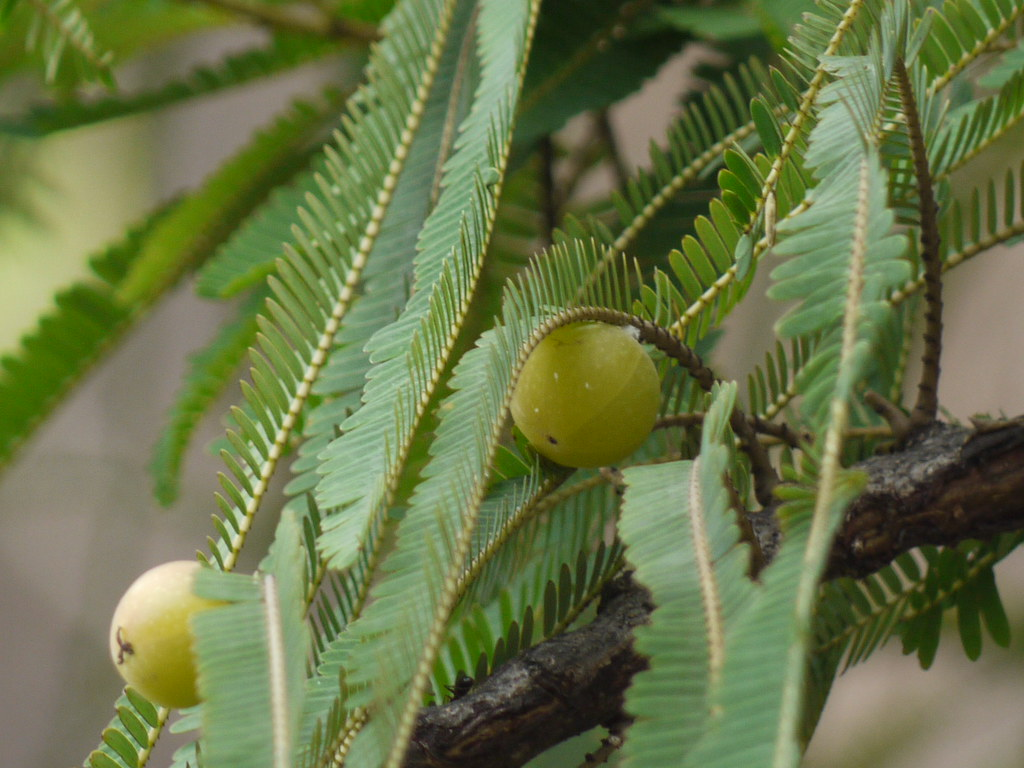
\includegraphics[width=0.46\linewidth]{media/amalaka_fruit}
    \hfill
    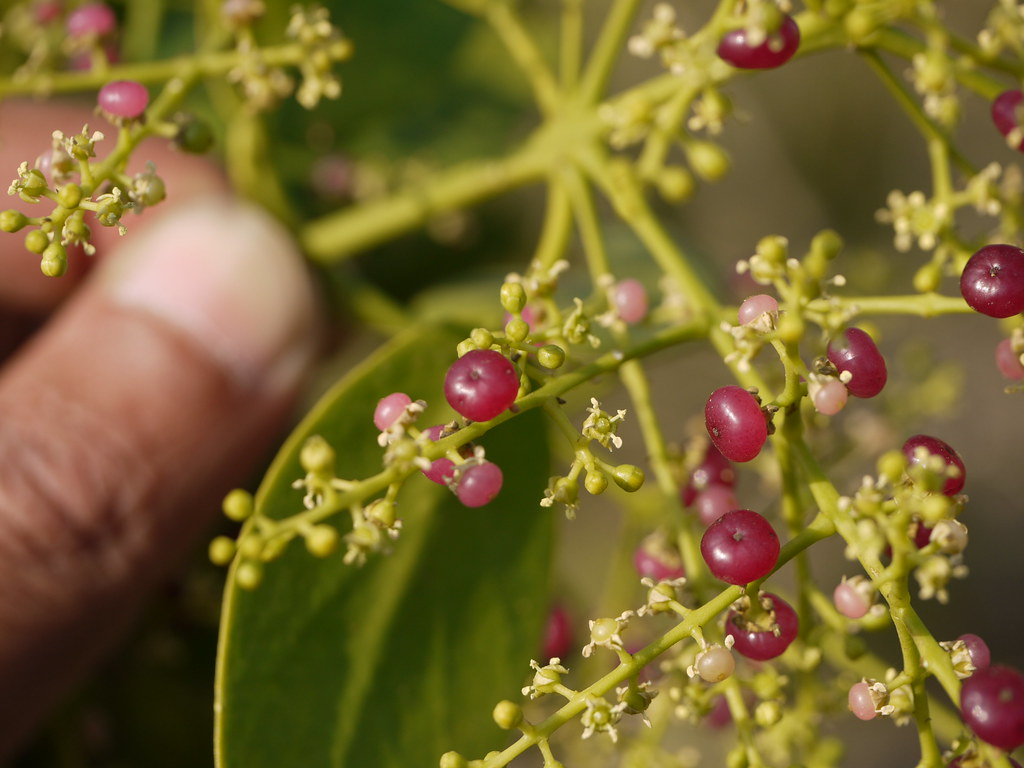
\includegraphics[width=0.46\linewidth]{media/pilu_fruit}
        \caption{Berries of the \egls{āmalaka} and \egls{pīlu}. Photos 
        courtesy of Dinesh Valke (CC-BY-SA).}
    \label{fig:pilufruit}
\end{figure}


\subsubsection{The origin of spiders}
\item[88cd--89]

This much has been declared to you.  Now I shall narrate the
\diff{authoritative} origin of spiders,\footnote{The vulgate's reading
    \dev{purāṇam} “ancient” is no doubt easier than \dev{pramāṇam}
    “authority,” but there is no support for it in the Nepalese
    manuscripts.} and in a general way the incurable and curable patient
    who has been bitten as well as the therapy and the \diff{distinctions
        to be made}.\footnote{The vulgate reads \dev{yathāviśeṣam} “according
        to their specifics,” qualifying the therapies.  The Nepalese version's
        \dev{viśeṣaṇam ca} “distinguishing, qualifying,” seems to be a
        separate topic for explanation.}
 
 \bigskip
    
\item[90--91, 92ab, 92ef]        

Once upon a time there was a good king called Viśvāmitra, “Friend to
All.”  He went to the ashram and somehow made Vaśiṣṭha, the best of
sages, angry.\footnote{On the legendary rivalry between these two
    figures, see \cite[Introduction, et passim]{sath-2015}.} Drops of
    sweat from that angry sage's forehead, as brilliant as the sun because
    of his countenance, reached the grass that had been cut
   and gathered by the sage for his
    cows.\footnote{\dev{niyetuḥ}, 3rd, pl., pf., \root \dev{yat},
        “reached, arrived,” is simplified in the vulgate to \dev{apatan} “they
        fell."
    
    The vulgate adds half a verse here giving a subject to the next
verb, \dev{varttante}: “From those were born these various,
terrible creatures with great poison” \Su{5.8.12cd}{592}.} They
started to damage the king's government and labours.\footnote{Ḍal.haṇa 
    cited a different origin myth, which itself began “others say\ldots .”}
    
    
\item[93]

Since the sage's drops of sweat reached the cut
(\emph{lūna}) grass, spiders (\emph{lūtā}) came into being.  And they
were sixteen in number.
    
 
 
 
 \subsubsection{Taxonomy of spiders}
 
 \item[94] 
 
 Spiders are traditionally said to be of two kinds:  those that are hard
 to treat and those that cannot be treated.  Amongst those, there are eight
 that are hard to treat and exactly the same number that should be 
 avoided.\footnote{ “Avoided” in the sense that treatment should not be 
 attempted.
     
     \citet{mana-2009} makes some spider identifications, but 
 their basis is not stated.}
 
 \item[95]
 
 They are traditionally said to be:
 \Gls{trimaṇḍalā}, 
 \Gls{śvetā-spider}, 
 \Gls{kapilā-spider}, 
 \Gls{pītikā-spider}, 
 \Gls{alaviṣa}, 
 \Gls{mūtraviṣa}, 
 \Gls{raktā-spider}, and the eighth is the
 \Gls{kasanā-spider}.
 
 \item[96]
 
 When bitten by one of these, there is headache and especially itching
at the site of the bite, and in particular maladies related to phlegm
and wind.
 
 \item[97]
 
 They are traditionally said to be:
 \label{sauvarnika-group}
 \Gls{sauvarṇikā},
 \Gls{lājavarṇā},
 \Gls{jālinī-spider},
 \Gls{eṇīpadī},
 \Gls{kṛṣṇamukhā},
 \Gls{agnimukhā},
 \Gls{kākāṇḍā}, and the eighth is the
 \Gls{mālāguṇī}.

\item[98]

If one is bitten by one of these, there is a sore at the site of the
bite and a flow of blood,\footnote{Elsewhere, \Dalhana{6.42.13}{718}
    glossed \dev{kṣataja} “wound-born, blood,” as \dev{ārtavarakta}
    “seasonal blood."} fever, a \se{dāha}{temperature} and diarrhoea and
    the illnesses caused by the three humours.
 
\item[99]
 There are also various kinds of boils and large rings, and large, soft, red and 
 dark swellings that move about.
 
\subsubsection{Specific symptoms and treatments}
 
 \item[100]
 
This is the generic characterization of the bites of all kinds of
spider.  I shall now describe their specific characterization,
together with the therapy. 


\paragraph{The \Gls{trimaṇḍalā} spider}

\item [101]

The bite of a \Gls{trimaṇḍalā} makes the blood bleed thick and dark. 
There is deafness, clouded vision, and a burning sensation in the
eyes.

\item[102]

In such a case, the root of \gls{arka}, \gls{rajanī}, \gls{nākulī} and 
\gls{pṛṣṇaparṇikā} are recommended in an errhine treatment and
\diff{for the massage of the feet} and in a collyrium. 


\paragraph{The \Gls{śvetā-spider}}

\item[103]

At the site of a bite of a \Gls{śvetā-spider}, a white, itchy spot
appears that comes with heat, fainting and fever, and causes  
\sse{visarpa}{spreading rash}a spreading, weeping rash and pain.

\item[104]

In such a case,a
\gls{candana}, 
\gls{rāsnā}, 
\gls{elā}, 
\gls{hareṇu},
\gls{nala}, 
\gls{vañjula}, 
\gls{kuṣṭha}, 
\gls{lāmajjaka}, 
\gls{vakra},
and \gls{nalada} are a healthy
antidote.\footnote{\Dalhana{5.8.105}{592} glossed several of these
    drugs and noted that others had different opinions.  In particular, he
    thought that \dev{vañjula} was \egls{jalavetasa} rather than
    \egls{vañjula}. But he also noted that Jejjaṭa thought it was
    \dev{kambukā}, an unidentified plant that Ḍalhaṇa thought should be
    interpreted as \egls{kiṇihī}.}



\paragraph{The \Gls{kapilā-spider}}

\item[105]

At the site of a bite of a \Gls{kapilā-spider}, there is a firm, coppery spot, the 
head feels heavy, and \diff{the person's eyes feel hot}.\footnote{The vulgate 
reads \dev{timiraṃ bhrama eva ca}, “a defect of vision and giddiness” 
\pvolcite{3}[97]{shar-1999}.}

\item[106]

The following remove the poison: 
\gls{padma},
\gls{padmaka},
\gls{kuṣṭha},
\gls{elā},
\gls{karañja},
\gls{kakubha},
\gls{tvac},
\gls{sthirā},
\diff{\gls{kampilya},}
\gls{apāmārga},
\gls{dūrvā}, and
\gls{brāhmī}.



\paragraph{The \Gls{pītikā-spider}}

\item[107]

At the site of a bite of a \Gls{pītikā-spider}, a hard, yellow spot develops, 
because of the yellow, accompanied by vomiting and fever,\footnote{Reading 
\dev{chardijvaraḥ} as a m.\ sg.\ dvandva. Cf.\ p.\,\pageref{masc-dvandva}.} 
sharp pain and the eyes may 
become red.

\item[108]

In such a case, the following are required:
\gls{kakubha},
\gls{uśīra},
\gls{muñja},
\diff{\gls{balvaja},}
\gls{vañjala},
%
\gls{kuśa},
\gls{kāśa},
\gls{vaṃśa},
\gls{kiṇihī},
\gls{śirīṣa},
\gls{kakubha},
and 
\gls{tvac}.\footnote{The repetition of \dev{kakubha} “arjun tree” suggests an 
error in the Nepalese transmission.}

\paragraph{The \Gls{alaviṣa} spider}

\item[109]

At the site of a bite associated with the \Gls{alaviṣa}, which is like a red circle, 
there are spots like \gls{sarṣapa} seeds.  It burns, the palate feels dry and 
there is a temperature.

\item [110]

In such a case, the antidote is
\gls{priyaṅgu},
\gls{hrīvera},
\gls{kuṣṭha},
\gls{lāmajjaka}, and
\gls{śatapuṣpā},
with the shoots of 
\gls{pippala}
and \gls{vaṭa}.


\paragraph{The \Gls{mūtraviṣa} spider}

\item[111]

The bite of a smelly \Gls{mūtraviṣa} spreads out, with black blood
accompanied by coughing and wheezing, vomiting and fainting, fever and
a burning feeling.

\item [112]

Famously, the poison can be destroyed by the following:
\gls{manaḥśilā},
\gls{madhuka},
\gls{kuṣṭha},
\gls{padmaka},
\gls{candana}, and
\gls{lāmajjaka}.


\paragraph{The \Gls{raktā-spider}}

\item[113]

The bite of the \Gls{raktā-spider} has pale, hot, \se{kleda}{weeping}
spots.  It can be identified because it is \se{coṣa}{dry} and red, with red edges.

\item[114]

In such a case, the treatment should be done with 
\gls{hrīvera},
\gls{candana},
\gls{uśīra},
\gls{padmaka},
\gls{arjuna},
\gls{śelu}, and the
bark of 
\gls{āmrātaka}.


\paragraph{The \Gls{kasanā-spider}}

\item[115]

The bite of the \Gls{kasanā-spider} makes cold, slimy blood flow.
There is also wheezing and coughing. The treatment is as stated for
the \Gls{raktā-spider}.\footnote{At this point, the vulgate has four
    verses that are not present in the Nepalese version.  They describe
    the symptoms and treatment of the bites of two further spiders, the
    \Gls{sauvarṇikā} and the \Gls{agnimukhā}.  \Dalhana{5.8.119}{593}
    reported that the commentator Gayadāsa thought the bites of the
    \Gls{sauvarṇikā} group (p.\,\pageref{sauvarnika-group}) were all incurable 
    so he only described them but described no treatment.}


 \item[120]
 
 The wise person should employ the bark of \gls{śleṣmātaka} in the case of 
 poisoning by any of them, and \gls{akṣīva} and \gls{pippala} in all 
 ailments.\footnote{\Dalhana{5.8.120}{593} understood the compound  
 \dev{akṣīvapippalam} as a tatpuruṣa, not a dvandva. I.e., “a \egls{pippala} 
     that comes from an \emph{akṣīva},” and he glosses the latter word as 
     \emph{mahānimba} or \emph{śobhāñjana}.
     
     Ḍalhaṇa also here quoted a passage from the lost work of
Ālambāyana (see pp.\,\pageref{alambayana1},
p.\,\pageref{alambayana2}): \dev{lūtāviṣeṣu sarveṣu
pānanasyāñjanādinā / prayojyaḥ pippalo'kṣīvajātaḥ
śelutvaco'thavā} “in all cases of spider-poison \gls{pippala}
that comes from \gls{akṣīva}, or else the bark of \gls{śelu},
should be used as drinks, errhines or ointments.”}

\subsubsection{Spider poisons hard to treat}
  
\item[121]

According to tradition, there are said to be eight spiders whose poison
is incurable.  Learn from me the symptoms of the potencies of these 
overpowering poisons.

\item[122]

The bite of the \Gls{sauvarṇikā} is dark, frothy, and smells like fish.  The 
coughing and wheezing, fever, thirst and fainting in this case are 
terrible.\footnote{\Dalhana{122}{593} glossed \dev{dhyāma} “dark” as 
“being the colour of burnt brick."}

\item[123]

When there is a bite by the \Gls{lājavarṇā}, blood runs out, dark and odorous. 
Heat, fainting, diarrhoea and a headache develop.

\item[124]

The bite of the \Gls{jālinī-spider} is terrible: it is striped and splits open. It 
causes paralysis, wheezing, increased \se{tamas}{gloominess} and dryness of 
the palate.\footnote{\Dalhana{5.8.124}{593} interpreted \dev{tamovṛddhi} 
as, “seeing darkness again and again."} 

\item[125]

The bite of the \Gls{eṇīpadī} has great heat and has the form of a black sesame 
seed.  There is thirst, fainting, fever and vomiting, accompanied by wheezing 
and cough. 

\item [125 add 1]

The bite of the \Gls{kṛṣṇamukhā} has black edges, a depressed middle
and very \se{coṣa}{dry}.  There is pallor, fainting, vomiting and
burning, accompanied by by wheezing and cough.\footnote{The following
    two verses are absent in the vulgate transmission, but deal correctly
    with the next two spiders listed above,
    p.\,\pageref{sauvarnika-group}, as having incurable bites.}

\item [125 add 2]

The bite of the \Gls{agnimukhā} is recognized as being burnt, with spots and 
with pain.  There is dryness, itching and horripilation, and suffering from heat 
and fever.

\item [126]

When someone is bitten by the \Gls{kākāṇḍā}, the bite is pale red and very 
painful. There is suffering from hiccuping, coughing, thirst, fainting, sleepiness, 
and pain in the heart.

\item [127]

The bite of the \Gls{mālāguṇī} is red, smells like smoke, and is extremely 
painful.  It splits open multiple times and is accompanied by burning, fainting, 
and fever. 

 \subsubsection{Curable and incurable}
 
\item [128]

Even for those cases that are incurable, the physician should apply
therapy, especially the elevation of the humours, with the exception
of excision.\footnote{The vulgate adds a compassionate phrase here,
    “after explaining [the incurability] to the patient.”  The vulgate
    also rules out cauterization.
    
    \Dalhana{5.8.128}{593} noted a variant reading \dev{asādhyānām api 
    cikitsitaṃ} that corresponds almost exactly to the Nepalese version.}

\item [129]

As soon as someone is bitten by a treatable spider, the wise physician
should excise the bite with a \se{vṛddhipatra}{big-leaf
    scalpel}.\footnote{On this scalpel, see
    \volcite{1}[232--235]{mukh-1913}, illustrated at 2, 121--122, and
    \cite[83--84]{wuja-2003}. Two forms of this scalpel were described by
    \Dalhana{1.8.3}{36--37} and are illustrated in that same edition: see
    Figure~\ref{fig:vrddhipatrascalpel}.}
\begin{figure}
    \centering
    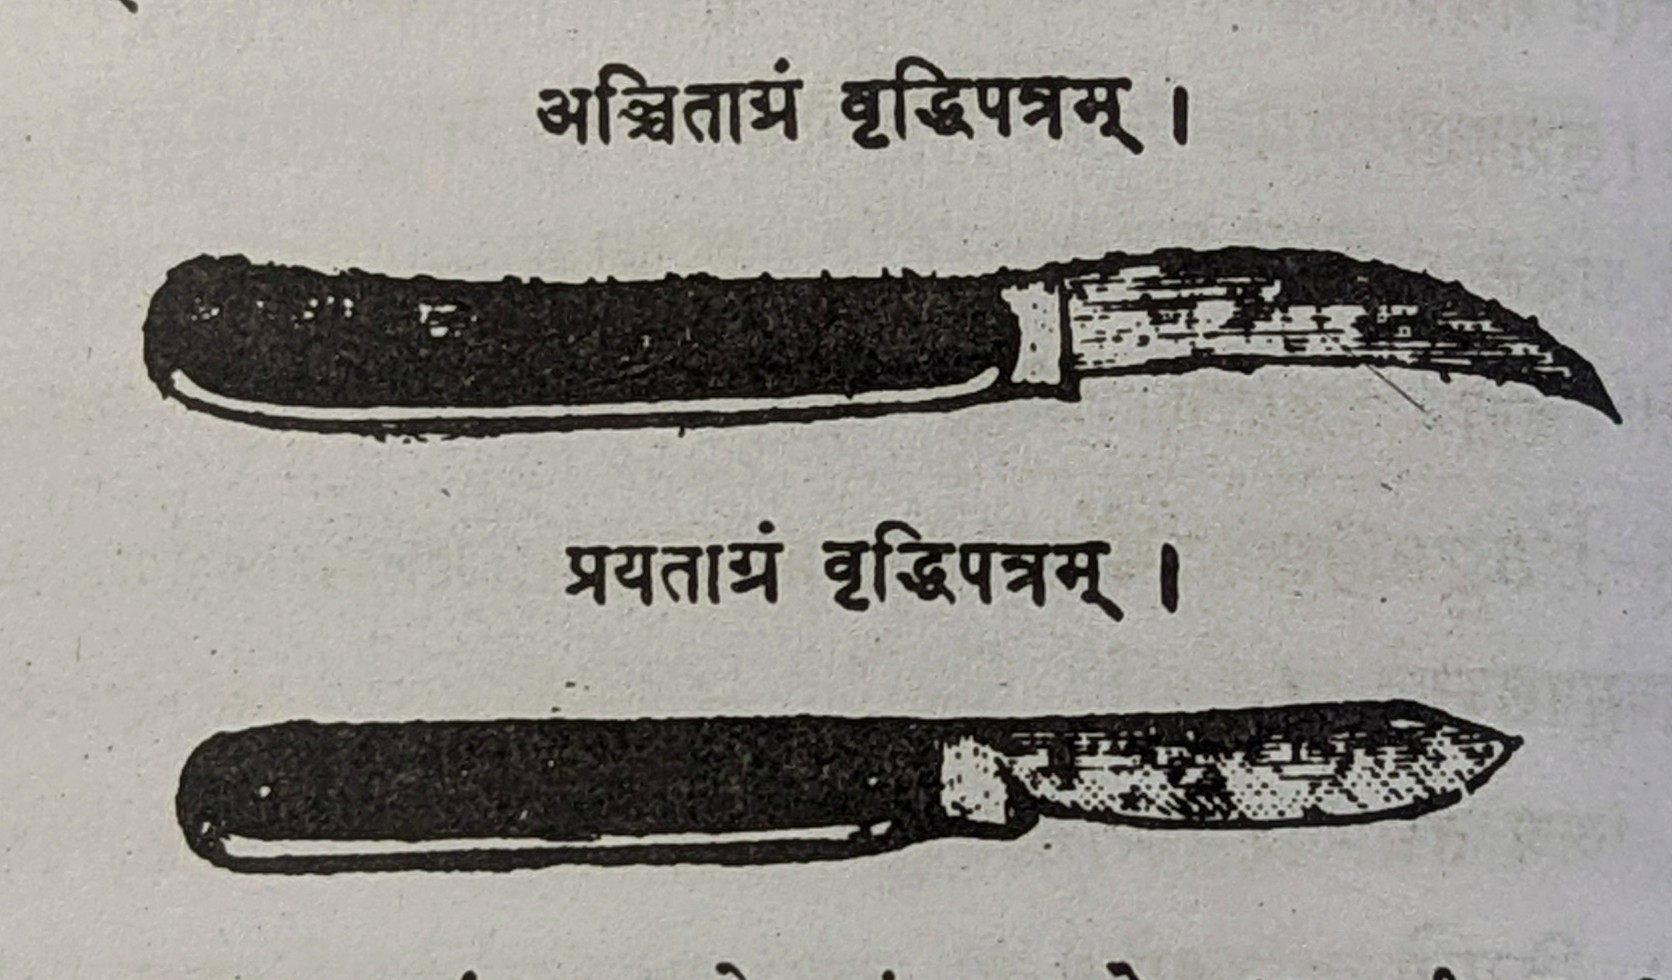
\includegraphics[width=0.7\linewidth]{media/vrddhipatra_scalpel}
    \caption{The big-leaf scalpels, as illustrated in \cite[36]{vulgate}.}
    \label{fig:vrddhipatrascalpel}
\end{figure}

\item[129 add 1]

To avoid spreading, one should cauterize with a very hot
\se{jamboṣṭha}{jambu-lip}.\footnote{This half-verse does not appear
    in the vulgate, but it was known to Ḍalhaṇa as a variant reading
    (\Dalhana{5.8.129}{593}).
    
    The “jambu-lip” is another surgical instrument, used for the
cauterization of fistula according to \Su{4.8.32}{440}.  Ḍalhaṇa
described it, loc.\ cit., as \dev{jambūphalasadṛśamukhāgrā
kṛṣṇapāṣāṇaracitā vartiḥ/} “a wick made out of black stone that
has a tip similar to the jambu fruit.”  See
\volcite{1}[159--160]{mukh-1913}, illustrated at 2, 74 (no.\,4).}

\item[131ab]

After that, one should smear on an antidote made of a mixture of honey and 
\gls{saindhava}. 

\item [133]



 % got to here




 \subsubsection{More therapies for spider poisoning}
 
 \item [130--134] xx
 
\subsection{General therapies for poisoning}

\item [135--139] xx

\subsection{End of the Kalpasthāna}

\item[140--143] xx
 
\end{translation}